\section{A Step-by-Step Guide to Conducting a Hypothesis Test}
\subsection{Step \#1}
\emph{Define your null and alternative hypotheses.} The null hypothesis is something that is already established and accepted as true, which we denote as $H_{0}.$ Also, suppose that the parameter value under the null hypothesis is $A_{0}.$

\subsection{Step \#2}
Take a sample, say of about 100 or 1000 people or event occurrences, and calculate the value of the estimator (for example, the average of the parameter such as average age, average pizza delivery time, average income, etc.). Let us assume that this value was $A_{m}.$

\subsection{Step \#3}
Calculate the standard normal $Z$-value:
\begin{align}
	Z=\dfrac{A_{m}-A_{0}}{\sigma/\sqrt{n}}
\end{align}

In the formula above, $\sigma$ is the standard deviation of the population or event occurrences, and $n$ is the number of subjects in the sample.

The probability associated with the $Z$-value calculated in Step $3$ must be compared with the significance level of the test to determine whether the null hypothesis will be accepted or rejected.

\subsection{Example}
A famous pizza restaurant claims that its delivery time is \emph{20 minutes}, with a standard deviation of 3 minutes. 

An independent market researcher claims that they are deflating the numbers to gain customers and that the average delivery time is actually \emph{21.2 minutes}.

Is their claim justified, or is the pizza business correct in its claim? \emph{Assume a significance level of $5\%$.}

Let us define the null and alternative hypotheses:
\begin{itemize}
	\item What the pizza business claims: $H_{0}:A_{0}=20.$
	\item What the researcher claims:
	$H_{a}: A_{0}>20.$
	\item Standard deviation (known): $\sigma=3.$
	\item Sample size: $n=64.$
	\item Significance level: $\beta=0.05.$
\end{itemize}

Let us calculate the $Z$-value:
\begin{align}
	Z=\dfrac{21.2-20}{3/\sqrt{64}}=3.2
\end{align}

Let us denote by $F$ the cumulative distribution function of a standard normal variable $N(0,1).$ 

We calculate the $p$-value corresponding to the value $Z=3.2$:
\begin{align}
	\texttt{p-value}&=1 - F(3.2)\\
	&=1-0.999312862062\\
	&= 0.000687137937916
\end{align}

This means that if the mean were $A_{0}=20,$ the probability that the sample mean would be $A=21.2$ is $\approx 0.069\%.$

Since we \emph{chose} a significance level $\beta=5\%,$ and $0.069\% < 5\%,$ we can reject the null hypothesis $H_{0}: A_{0}=20.$

\begin{figure}
	\centering
	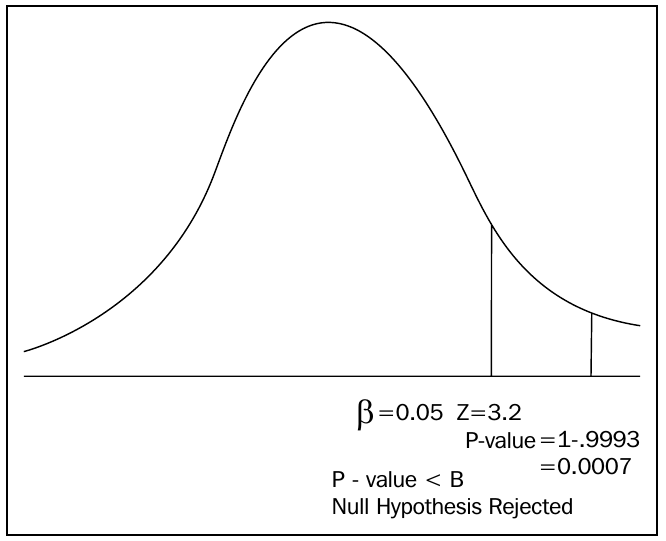
\includegraphics[height=5cm,keepaspectratio=true]{./images/kum0405.png}
	% kum0405.png: 0x0 pixel, 300dpi, 0.00x0.00 cm, bb=
	\caption{The null hypothesis is rejected because the $p-$value is less than the significance level $\beta$.}
	\label{fig:3.8.1}
\end{figure}
